\documentclass{article} 
\usepackage{amssymb, amsfonts, amsmath}
\usepackage{graphicx}
\begin{document}
{ \Large \bf 
Finding the line of least variance\\

}

A problem in sketch recognition is determining the orientation of a sketch. A detector should detect both a diagonally rotated rectangle and an axis-aligned rectangle. In general, a detector should detect sketches invariant of orientation. 
\begin{figure}[htbp]
\begin{center}
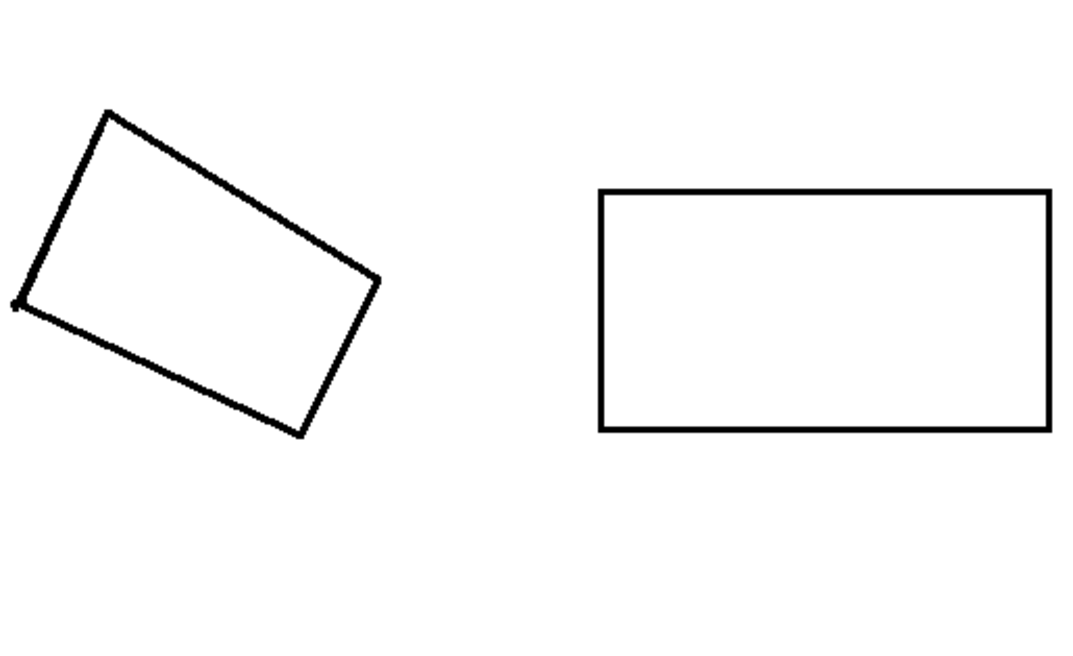
\includegraphics[scale=.5, clip=true, trim=0 100 0 50]{example1}
\caption{Example 1: Diagonal vs. axis aligned rectangle}
\label{ex1}
\end{center}
\end{figure}

An intuitive method for making a detector orientation invariant is sketch via pre-processing. In this pre-processing step, the coordinate frame of a given sketch is transformed to be axis-aligned with respect to that sketch.

\begin{figure}[htbp]
\begin{center}
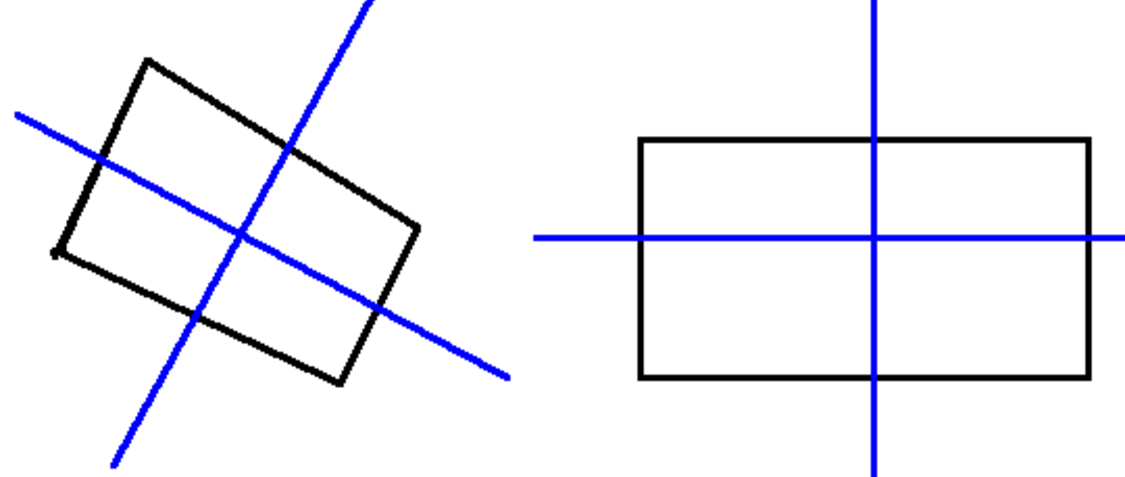
\includegraphics[scale=.5]{example2}
\caption{Example 2: Preprocess axis transform}
\label{ex2}
\end{center}
\end{figure}

After finding this transform, we can re-compute the parametric representation of the sketch through time in the new coordinate plane as input to the detector. This allows the detector to only detect axis-aligned versions of sketches. The question now arises, how do we find this `ideal' coordinate transform? 

Observing that our axis will always be perpendicular from each other, we can simplify this problem to finding a single `good' axis. Lets find the line (axis) that is closest to all points using the L-2 metric. This line will be parallel to the direction of maximum variance in the shape. 

\begin{align*}
\min_{x_1,x_0,y_1,y_0} & \sqrt{\sum_{i=2}^{n+1} \left( \frac{(x_1 - x_0)(y_0 - y_i) - (x_0 - x_i)(y_1 - y_0)}{\sqrt{(x_1 - x_0)^2 + (y_1 - y_0)^2}}\right)^2}\\
\text{Fix} \quad & x_1 = 1, x_0 = 0\\
 = \min_{y_1,y_0} & \sqrt{\sum_{i=2}^{n+1} \frac{((y_0 - y_i) + x_i(y_1 - y_0))^2}{1 + (y_1 - y_0)^2}}\\
= \min_{y_1,y_0} &\sum_{i=2}^{n+1} \frac{((y_0 - y_i) + x_i(y_1 - y_0))^2}{1 + (y_1 - y_0)^2}\\
\text{Observe that} \quad & m = \frac{y_1 - y_0}{x_1 - x_0} = y_1 - y_0, \text{ and } b = y_{\text{intercept}} = y_0.\\
= \min_{m,b} &\sum_{i=2}^{n+1} \frac{(b - y_i + mx_i)^2}{1 + m^2}\\
= \min_{m,b} &\frac{1}{1+m^2}\sum_{i=2}^{n+1}(y_i - mx_i - b)^2\\
\end{align*}
Ok great so now we have an optimization problem which we would like to find an analytical closed form solution to. We will do this by setting the partial derivatives to zero.
\begin{align*}
 0 & = \frac{\partial}{\partial b}\left(\sum_{i=2}^{n+1}\frac{(y_i - mx_i - b)^2}{1+m^2}\right)\\
 0 & = \sum_{i=2}^{n+1}\frac{-2(y_i - mx_i - b)}{1 + m^2}\\
 0 & = \sum_{i=2}^{n+1}(y_i - mx_i - b)\\
 \bar{y} & = m \bar{x} + b\\
\end{align*}

\begin{align*}
0 & = \frac{\partial}{\partial m}\left(\sum_{i=2}^{n+1}\frac{(y_i - mx_i - b)^2}{1+m^2}\right)\\
0 & = \sum_{i=2}^{n+1}\frac{-2(b + mx_i - y_i)(bm - my_i - x_i)}{(1+m^2)^2}\\
0 & = \sum_{i=2}^{n+1}(b + mx_i - y_i)(bm - my_i - x_i)\\
0 & = \sum_{i=2}^{n+1}(b + mx_i - y_i)(my_i + x_i)\\
0 & = \sum_{i=2}^{n+1}(\bar{y} - m\bar{x} + mx_i - y_i)(my_i + x_i)\\
0 & = \sum_{i=2}^{n+1}((\bar{y} -y_i)- m(\bar{x} - x_i))(my_i + x_i)\\
0 & = \sum_{i=2}^{n+1}(my_i(\bar{y} -y_i)- m^2y_i(\bar{x} - x_i) + x_i(\bar{y} -y_i) - mx_i(\bar{x} - x_i))\\
\end{align*}

\end{document}